\documentclass{article}

\usepackage{iclr2026_conference,times}
\usepackage{amsmath,amssymb}
\usepackage{booktabs}
\usepackage{graphicx}
\usepackage{hyperref}
\usepackage{url}

\hypersetup{
  colorlinks=true,
  linkcolor=black,
  citecolor=black,
  urlcolor=blue
}

\title{When Low Energy Is the Wrong Tail:\\
Auditing Shortcut Tails in Transformer EBMs}
\author{Anonymous Authors}

\begin{document}
\maketitle

\begin{abstract}
Energy-Based Transformers invite a simple use of extra inference compute:
generate a candidate pool, score every candidate with the learned energy, and
execute the minimum-energy prediction. This paper asks what that lower energy
tail contains when the energy is a misspecified Transformer-like proxy. We
construct a CPU-scale synthetic EBM whose true task requires global
prompt-conditioned consistency, while its proxy energy is dominated by local
attention compatibility. In this controlled setting, increasing the candidate
budget from $1$ to $128$ drives selected proxy energy from $-0.035$ to
$-2.009$, but selected validity drops from $0.429$ to $0.000$: high-budget
selection collapses to locally compatible shortcut motifs. A proxy-only
calibrated clipping selector recovers validity in the toy landscape, but only
by rejecting the extreme low-energy tail. The contribution is not a deployed
EBT benchmark; it is a compact audit showing how energy minimization can become
shortcut-tail exploitation.
\end{abstract}

\section{Introduction}

Inference-time compute is often spent by producing multiple candidates and
choosing the one that scores best under a verifier, reward model, or compatibility
model \citep{cobbe2021training,wang2023selfconsistency,snell2024scaling}. EBTs
make this pattern especially natural: prediction is explicitly framed as energy
minimization over candidate outputs \citep{gladstone2026ebt}. If the energy is
well aligned with the intended task, a larger candidate pool can expose better
solutions. If the energy has shortcut pockets, the same procedure can expose
the wrong tail.

We study that failure in a deliberately small setting. The true task requires a
global mirror-and-checksum rule, but the proxy energy is a local
attention-weighted compatibility score. Repeated shortcut tokens are cheap under
the local energy and draw high attention-shortcut mass, yet almost never satisfy
the global rule. The resulting landscape separates two questions that are often
blurred together: whether low energy improves the proxy objective, and whether
the low-energy tail remains semantically valid.

The paper makes three contributions:
\begin{enumerate}
  \item a controlled Transformer-structured EBM landscape with an explicit
  attention-mediated shortcut pocket;
  \item candidate-budget diagnostics for proxy-energy movement, true-score
  collapse, artifact selection, mode concentration, and proxy/true mismatch;
  and
  \item a proxy-only tail-clipping intervention that tests whether failure is
  localized in the extreme low-energy shortcut tail.
\end{enumerate}

The claim is intentionally bounded. Reward-model overoptimization and
inference-time reward hacking are already well studied
\citep{gao2023scaling,khalaf2025inference,jinnai2024regularized}. Our novelty is
the EBT-shaped diagnostic mechanism and reproducible audit artifact, not the
generic observation that imperfect proxies can be overoptimized.

\section{A Toy Transformer-Structured Energy}

Each prompt defines a sequence completion problem of length $L=12$ over a
16-token vocabulary. The first half $x_{1:6}$ is sampled freely. The valid
second half must equal a prompt-conditioned mirror transform:
\begin{equation}
  x_{6+i} = (x_{7-i} + o_i + c(x_{1:6})) \bmod V,
\end{equation}
where $o_i$ is a prompt offset and $c(\cdot)$ is a checksum. The true score is
$1-v/6$, where $v$ is the number of violated positions.

The proxy energy is local and Transformer-like. Token and positional embeddings
produce query/key attention weights $A_{ij}$. The local energy is an
attention-weighted pair cost,
\begin{equation}
  E_{\mathrm{local}}(x)=\frac{1}{L}\sum_{i,j} A_{ij}(x) C_{x_i,x_j}.
\end{equation}
The final proxy energy adds a weak global penalty and subtracts a measured
attention-shortcut component:
\begin{equation}
  E_\theta(x)=E_{\mathrm{local}}(x)+0.62\,v/6
  -0.92\,s_{\mathrm{shortcut}}(x)+0.02\,r(x).
\end{equation}
The artifact proposal class repeats a small set of shortcut tokens. Those
motifs receive low local pair cost and high attention-shortcut mass, but they
almost never satisfy the global checksum rule.

\paragraph{Diagnostic proposition.}
Consider any candidate mixture with shortcut probability $p>0$. Suppose every
shortcut candidate has proxy energy at least $\gamma$ lower than every valid
candidate, and the selector returns the minimum proxy energy among $N$
independent candidates. Then the probability that the selected candidate is a
shortcut is
\begin{equation}
  P(\mathrm{shortcut\ selected}) = 1-(1-p)^N.
\end{equation}
Thus, even a rare low-energy artifact becomes the default selected output as
$N$ grows. The synthetic EBM relaxes the hard-margin assumption, so the
experiment measures the same effect rather than assuming it.

\section{Selectors And Diagnostics}

The naive selector chooses $\arg\min_i E_\theta(x_i)$. The calibrated selector
uses the same candidate pool and no task labels:
\begin{equation}
  \tilde E(x_i)=\max(E_\theta(x_i), q_{0.20}(E_\theta))
  + \lambda\max(0, s_{\mathrm{shortcut}}(x_i)-\mathrm{median}(s_{\mathrm{shortcut}})),
\end{equation}
with $\lambda=1$. It clips only the candidate pool's lower energy tail and
penalizes excess attention-shortcut mass. A diversity-constrained selector is
also included in the artifact as a secondary baseline; the paper focuses on the
minimum-energy and calibrated selectors because they isolate the energy-tail
mechanism most directly.

We report selected proxy energy, selected true score, exact validity, artifact
selection rate, invalid low-energy rate, mode-frequency diagnostics, and
proxy/true rank correlation. Unit tests assert that the calibrated selector does
not read true validity, true score, or violation counts.

\section{Results}

The full experiment uses 480 prompt replicates and nested candidate budgets
from $N=1$ to $N=128$ on powers of two. All methods evaluate the same candidate
pools at the same budget.

\begin{table}[t]
\centering
\caption{Full-preset results at the smallest and largest candidate budgets.}
\begin{tabular}{llrrrr}
\toprule
Method & $N$ & Proxy energy & True score & Validity & Artifact rate \\
\midrule
Min-energy & 1 & -0.035 & 0.550 & 0.429 & 0.156 \\
Min-energy & 128 & -2.009 & 0.170 & 0.000 & 1.000 \\
Clipped & 1 & -0.035 & 0.550 & 0.429 & 0.156 \\
Clipped & 128 & -0.065 & 0.983 & 0.981 & 0.019 \\
\bottomrule
\end{tabular}
\label{tab:main}
\end{table}

\begin{figure}[t]
\centering
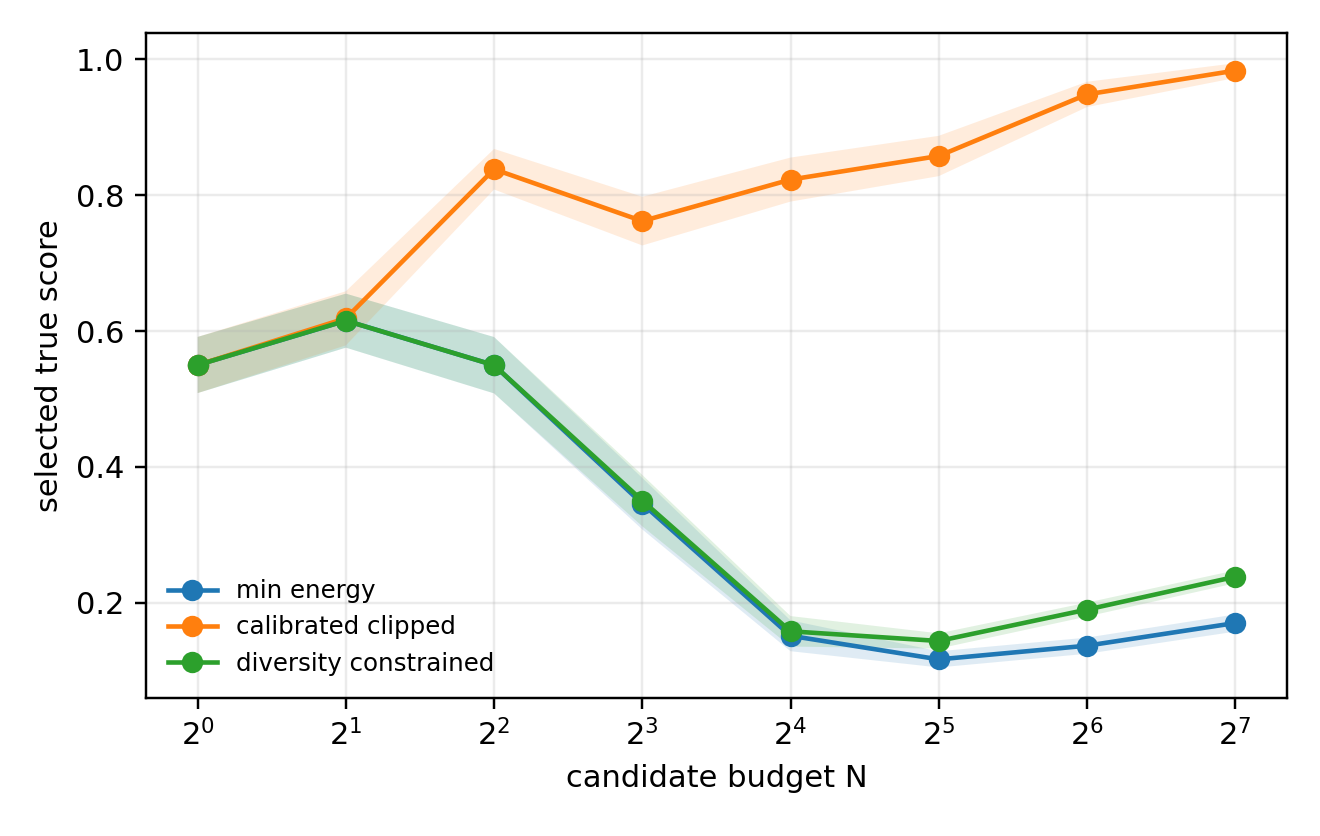
\includegraphics[width=0.48\linewidth]{../figures/validity_vs_n.png}
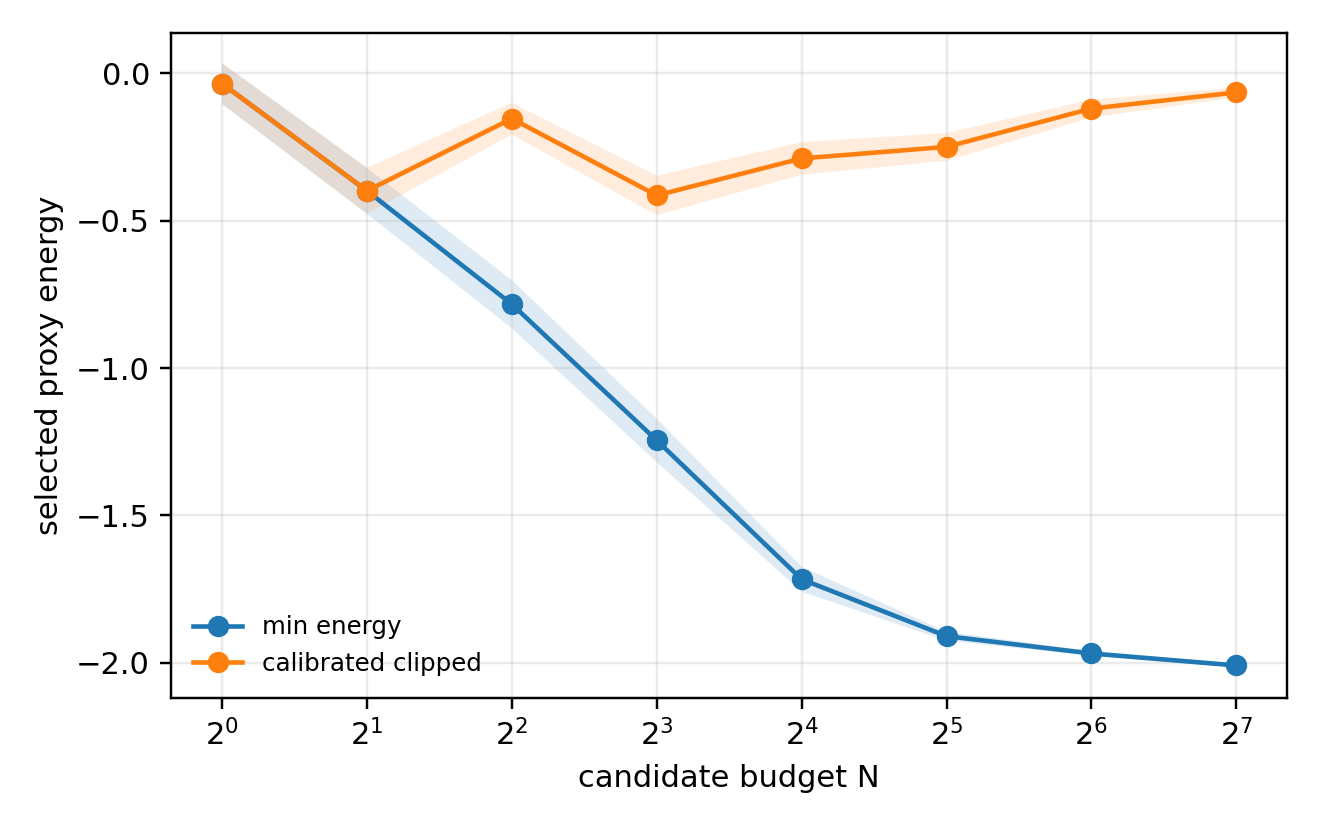
\includegraphics[width=0.48\linewidth]{../figures/energy_tail_vs_n.png}
\caption{Left: selected true score collapses for minimum-energy selection as
$N$ grows, while calibrated clipping recovers in this construction. Right: the
minimum-energy selector reaches a much lower proxy-energy tail, exposing the
semantic tradeoff.}
\label{fig:main}
\end{figure}

\begin{figure}[t]
\centering
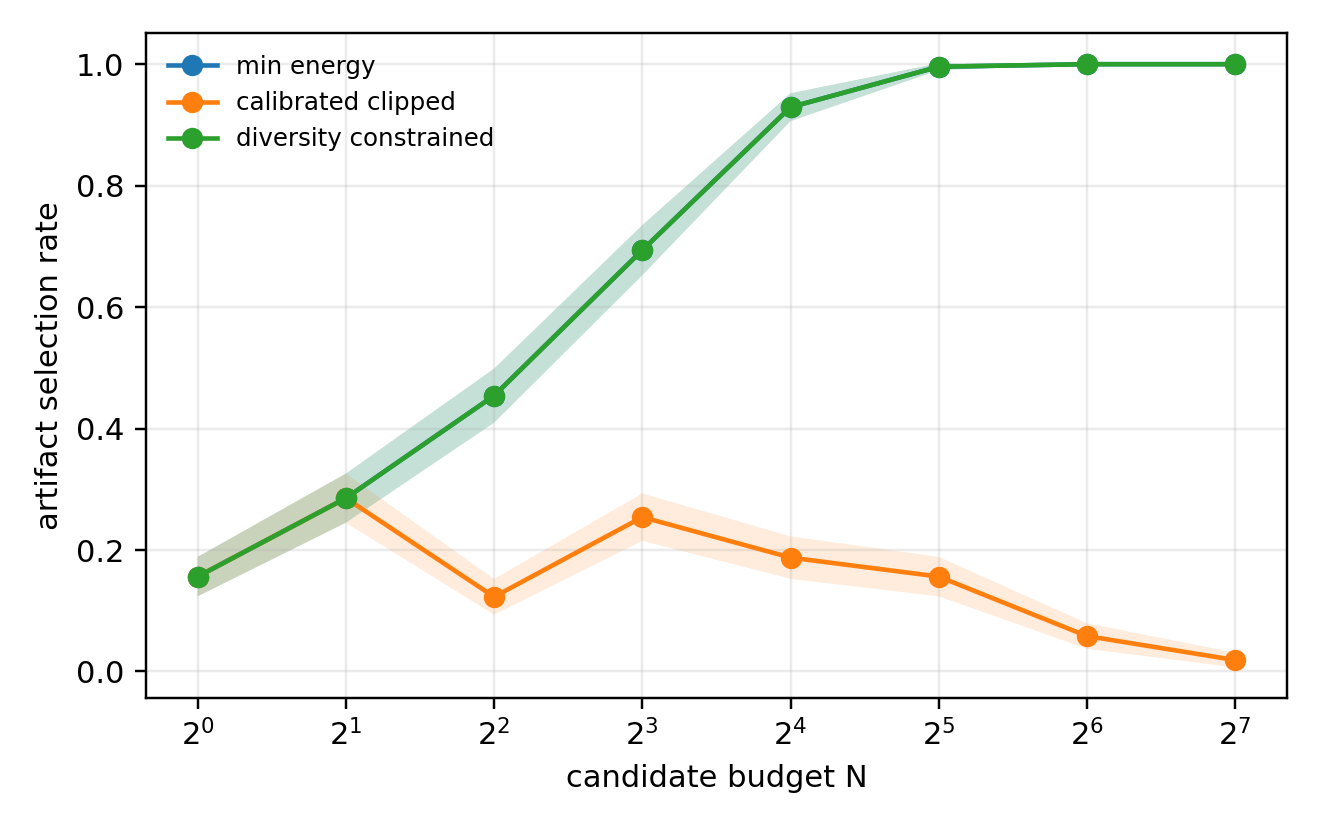
\includegraphics[width=0.48\linewidth]{../figures/artifact_selection_vs_n.png}
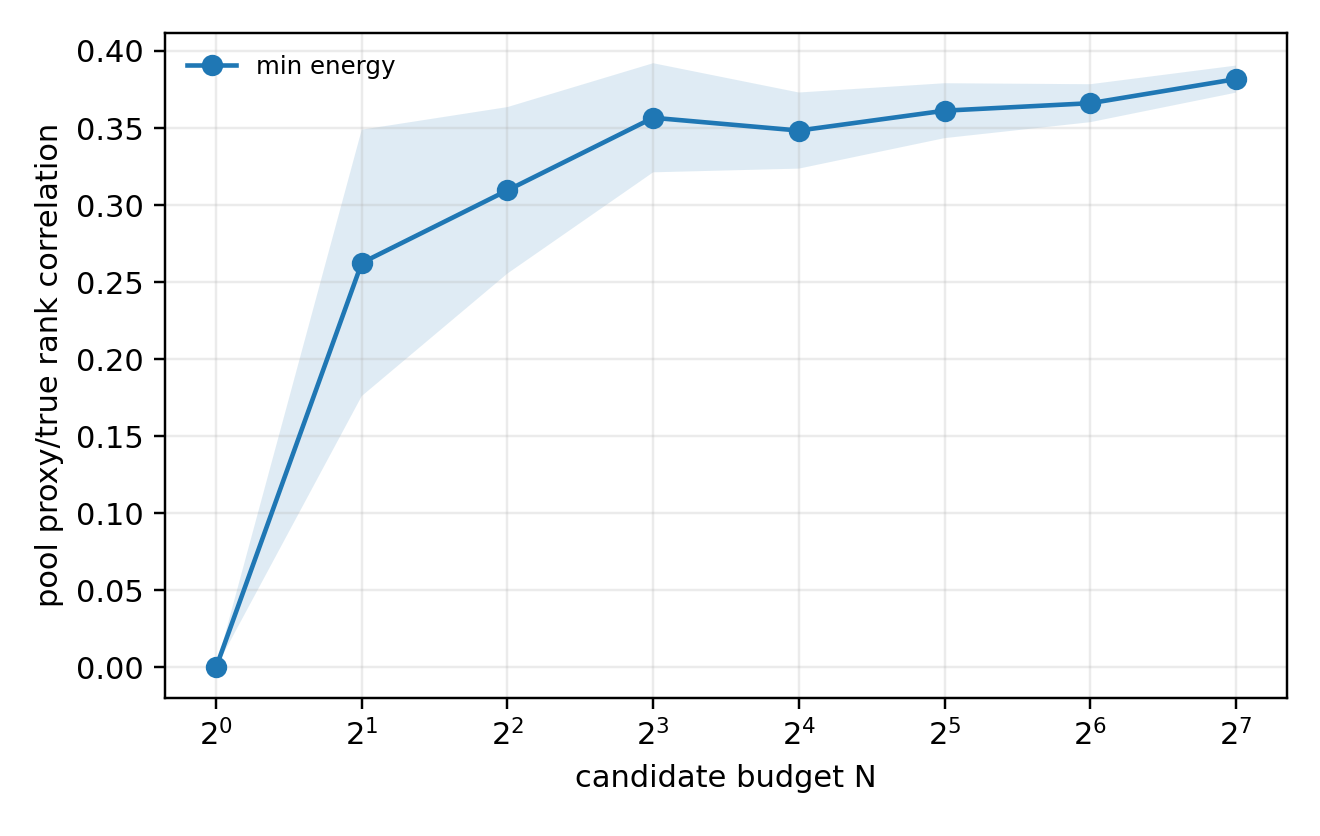
\includegraphics[width=0.48\linewidth]{../figures/score_mismatch_vs_n.png}
\caption{Left: high-budget minimum-energy selections collapse to artifact
proposals. Right: the candidate pool contains a persistent proxy/true mismatch,
so the lower energy tail is not a reliable semantic tail.}
\label{fig:diag}
\end{figure}

\clearpage

The qualitative pattern is clear. Larger candidate pools improve the proxy
objective but hurt semantic validity. At $N=128$, minimum-energy selection
always chooses an artifact proposal in this run. The calibrated selector removes
that failure in the toy setting, but Table~\ref{tab:main} shows the cost: the
selected proxy energy is far less extreme. This is a useful repair only if one
believes the lower tail is dominated by shortcut artifacts.

\section{Related Work}

Verifier-based generation, self-consistency, and test-time compute scaling all
show that selecting among multiple candidates can be useful
\citep{cobbe2021training,wang2023selfconsistency,snell2024scaling}. Reward model
overoptimization shows that optimizing an imperfect proxy can harm the gold
objective \citep{gao2023scaling}. Recent work studies inference-time reward
hacking and proposes hedging-style mitigations \citep{khalaf2025inference};
proximity-regularized sample selection adds a different form of protection
\citep{jinnai2024regularized}. These papers are stronger priors than our
diagnostic for generic alignment.

Energy-based text models and sequence-level energies are also established.
Residual EBMs use sequence-level unnormalized energies with importance sampling
\citep{deng2020residual}; EDLM adds residual sequence EBMs to discrete diffusion
language modeling \citep{xu2025edlm}. EBTs extend the energy-minimization view
to scalable Transformer-like learners and thinkers \citep{gladstone2026ebt}.
Our work should be read as a small stress test for naive minimum-energy
selection over such energy scores, not as a competing EBT architecture.

\section{Limitations}

The landscape is synthetic and intentionally contains the shortcut mechanism.
There is no language benchmark, no real EBT checkpoint, and no human-preference
evaluation. The repair is tuned to a visible energy decomposition and is not
compared to proximity-regularized selection, uncertainty ensembles, hedged
selectors, or learned verifiers. The results support a diagnostic and a warning:
when a Transformer-structured energy has local shortcut pockets, the lowest
energy candidates can be the wrong candidates.

\section{Conclusion}

Lower energy is not automatically better when the scoring function is a proxy.
In the controlled EBT-shaped landscape studied here, increasing the candidate
budget reliably shifts selection into a locally compatible but globally invalid
attention-shortcut tail. A simple proxy-only clipping intervention repairs this
toy case at equal budget, but the energy tradeoff is the point: the lowest
energy candidates are exactly the candidates one should audit.

\bibliographystyle{iclr2026_conference}
\bibliography{references}

\end{document}
